% Appendix Template

\chapter{Grafana} % Main appendix title

\label{AppendixB} % Change X to a consecutive letter; for referencing this appendix elsewhere, use \ref{AppendixX}

\lhead{\emph{Grafana}} % Change X to a consecutive letter; this is for the header on each page - perhaps a shortened title

\begin{figure}[b]
	\centering
		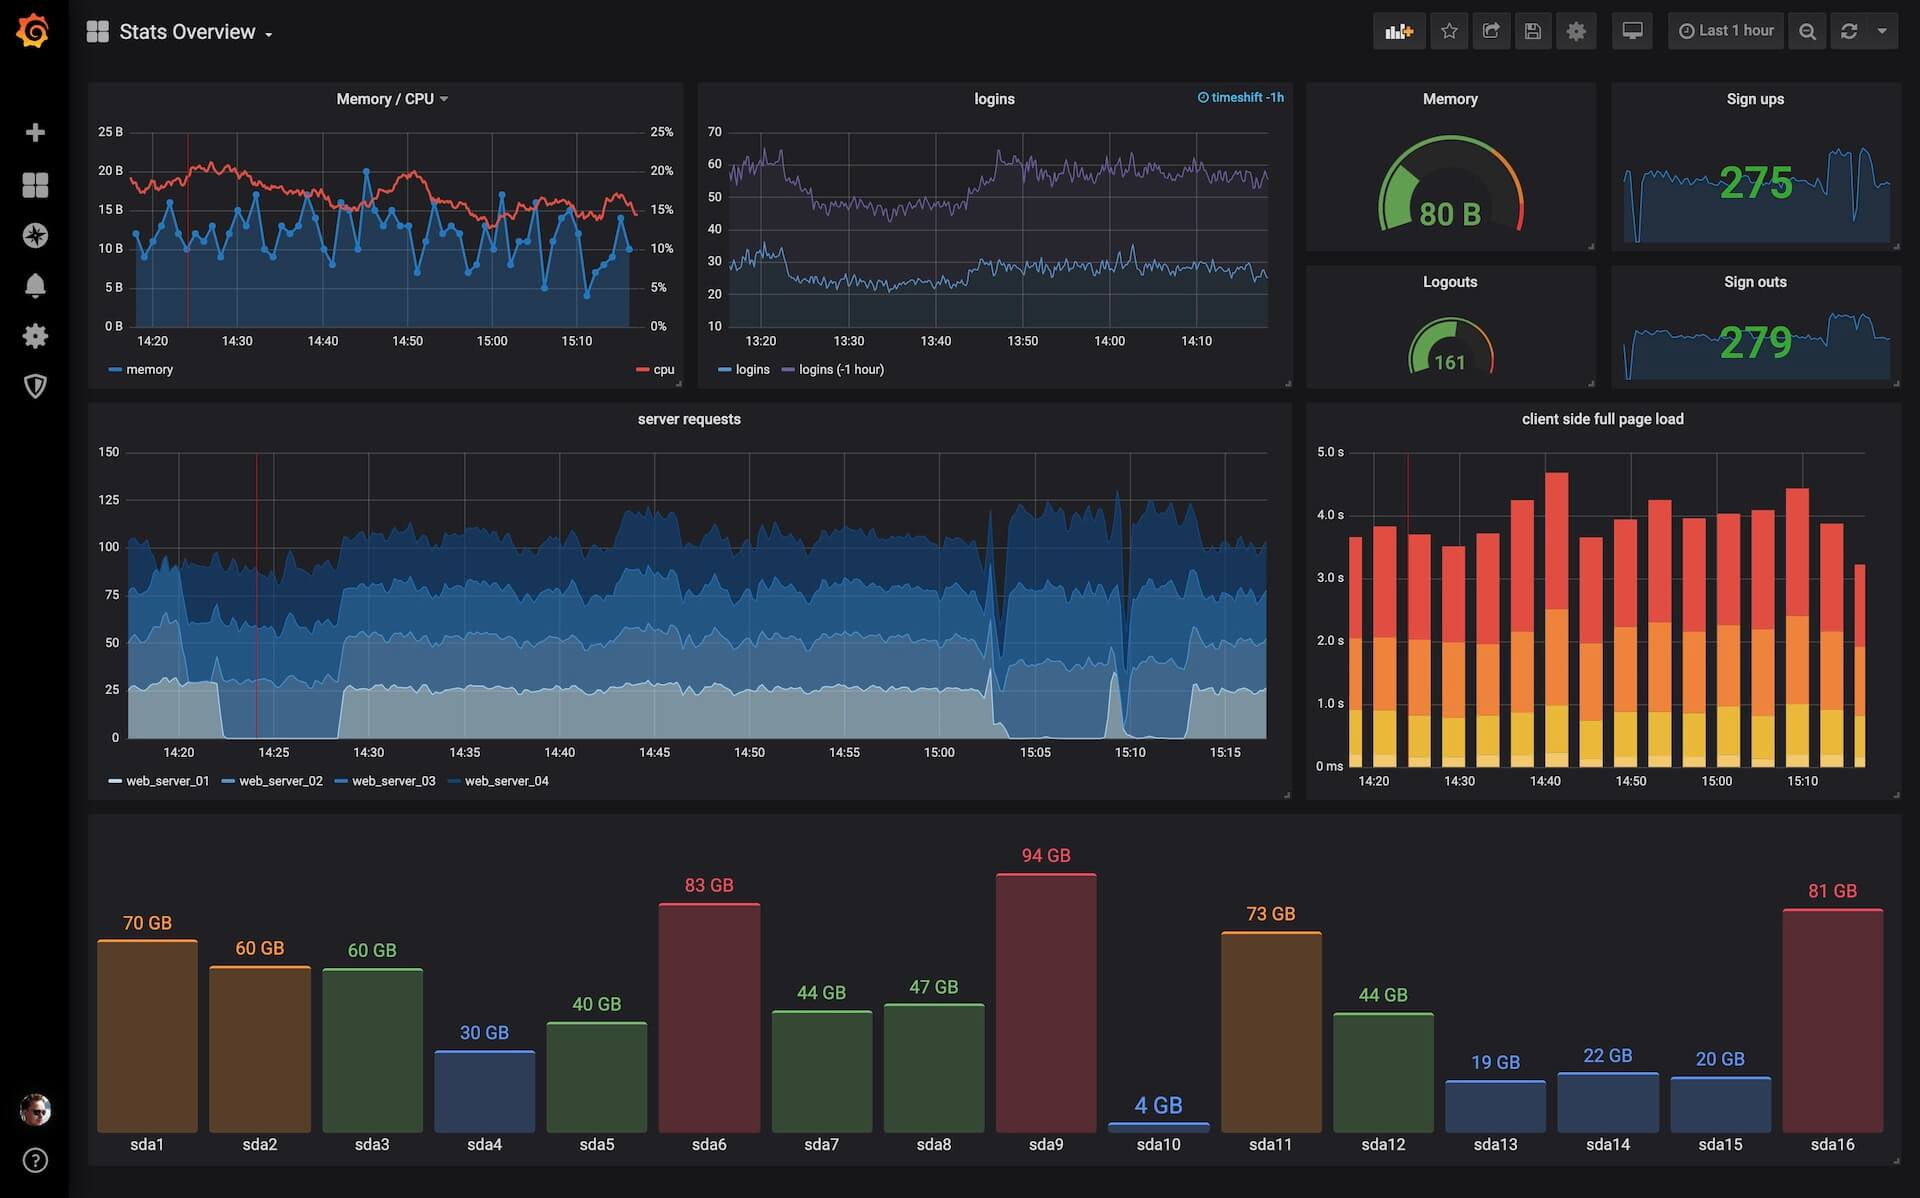
\includegraphics[width=1.0\columnwidth]{Figures/grafana.jpg}
		\rule{35em}{0.5pt}
	\caption[Grafana]{Grafana}
	\label{fig:Grafana}
\end{figure}

Grafana (Figure \ref{fig:Grafana}) is a multi-platform open source analytics and interactive visualization software available since 2014. It provides charts, graphs, and alerts for the web when connected to supported data sources. It is expandable through a plug-in system. End users can create complex monitoring dashboards using interactive query builders.

As a visualization tool, Grafana is a popular component in monitoring stacks, often used in combination with time series databases such as Prometheus and Graphite; monitoring platforms such as Sensu, Icinga, Zabbix, Netdata, and PRTG; SIEMs such as Elasticsearch and Splunk; and other data sources.

In this thesis, Grafana is used extensively for graphing the visualizations made using SQL queries using its MySQL plugin.
As part of my thesis, I have written a library for automating dashboard creation in Grafana through the provided HTTP API documentation so that the system can autogenerate
relevant dashboards and graphs after having analysed the MySQL data using SQL queries.

A link to the GitHub repository with the library is provided:
\newline
\url{https://www.github.com/sankalp-sangle/MySQL-Grafana.git}
\newline
A link to the GitHub repository for Grafana is provided:
\newline
\url{https://www.grafana.com}


